\documentclass[a4paper]{article}
\usepackage[utf8]{inputenc}
\usepackage{relsize}
\usepackage{url}


\title{Behavioral Model Editor\\ {\smaller Another title}}

\author{\emph{Written by:} Omar El Alfy}

\date{\today}

\usepackage{natbib}
\usepackage{graphicx}

\newcommand{\CADENA}{\textsc{Cadena}-e}

\begin{document}

\maketitle



\begin{abstract}
  The original \textsc{Cadena} featured only structural
  modeling. However, a generic, abstract, behavioral specification in
  form of activity graphs will mark an important step towards pure
  model driven development (where actual coding can be reduced to a
  minimum or even eliminated). In this project, graph-based and
  form-based editors for behavioral modeling based on lightweight
  process coordination will be implemented.
\end{abstract} 



\newpage

\section{Introduction}

A graph-based editor based on lightweight process coordination is a service-oriented approach that is easy to use and customize even for non-programmers to develop a services or an applications. Implementing this graph editor as an eclipse plug-in using Eclipse Modeling Framework (EMF) for defining the graph's model and Graphical Modeling Framework (GMF) for implementing the plug-in view and interface based on the graph's model generated by the EMF.

\section{Eclipse Modeling Framework (EMF)}

EMF is an eclipse modeling framework and code generation for building applications based on structured data  model, this model is described in XML Metadata Interchange (XMI). EMF uses this XMI model to produce it's Java classes, and generate it's editor. To create a model based on a digram EMF requires Ecore Tools SDK to be installed. The Ecore diagram has defined elements that could used simply by dragging and doping, elements like Eclass that represents a Java class, EAttribute represents an attribute in the class, ERefernce represents a relation between two classes and EData type represents the type of an attribute.

\section{Graphical Modeling Framework (GMF)}

GMF is an eclipse framework that creates a graphical editor based on meta models following Model View Controller architecture (MVC). GMF uses EMF for the model and Graphical Editing Framework (GEF) as a Controller. 

\begin{figure}[htp]
\centering
\includegraphics[width=0.8\linewidth]{GMFDashboard}
\caption{GMFDashboard}
\label{GMFDashboard}
\end{figure}

GMF has six steps to create a generated graphical editor using the GMF dashboard in the figure above, starts with the creating the Domain Model using the Ecore Tools SDK then deriving the Domain Gen Model (.genmodel) this file is used by EMF to generate the editor. Then derive two files Graphical Def Model (.gmfgraph) and Tooling Def Model (.gmftool). The  Graphical Def Model is used to define the graphical elements and the Tooling Def Model is used to define the palette of tools that are used in the editor. After that combining the files to create Mapping Model (.gmfmap) that links the domain model, the graphical model (.gmfgraph) and the tooling model (.gmftool). The last step is generating the Diagram Editor Gen Model (.gmfgen).


\section{Graph Model}

\begin{figure}[htp]
\centering
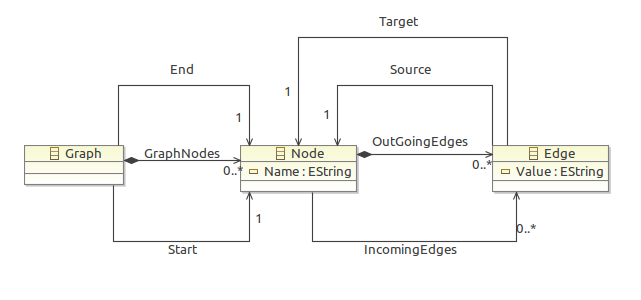
\includegraphics[width=0.8\linewidth]{GraphModel}
\caption{GraphModel}
\label{GraphModel}
\end{figure}

This graph model is a directed graph model that has a class graph containing a list of node, has one start node and one end node. Each node contains list of outgoing edges and incoming edges. Each edge has one source node and one target node. These are the characteristics that define the model for the graph that the GMF uses to generate the editor with some customizing in the tooling model and the graphical model. This model will be updated to add a feature that allows the graph to have more than one start and end node, also node types to allow the graph to run nodes in parallel and a feature that allows a each node to contain a graph and assigning the graph's output to the parent node's output. 

\newpage
\section{References}

url={http://met.guc.edu.eg/Repository/Faculty/Publications/372/2008.ISOLA.pdf}\\
url={http://sws-challenge.org/workshops/2006-Stanford/papers/06.pdf}\\
url={https://www2.lirmm.fr/lirmm/interne/BIBLI/CDROM/INFO/2012/ICSE_2012/icse2012/icsews12topi/p7-naujokat.pdf}
url={http://www.vogella.com/articles/EclipseEMF/article.html}\\
url={http://wiki.eclipse.org/Graphical_Modeling_Framework/Tutorial/Part_1}\\
url={http://www.kermeta.org/docs/fr.irisa.triskell.kermeta.samples.fsm.documentation/build/html.single/KerMeta-Create-FSM-Graphical-Editor-With-GMF/}\\
url={http://www.eclipse.org/modeling/emf/}\\
url={http://en.wikipedia.org/wiki/Graphical_Modeling_Framework}\\
url={http://en.wikipedia.org/wiki/Graphical_Editing_Framework}\\



\end{document}
